\chapter{Enregistrement des données}
\label{chap:Enregistrement des données}

\section{Les enjeux de la journalisation}

L'enregistrement des données circulant sur le réseau correspond à plusieurs besoins. En effet, avec la nouvelle architecture, les étudiants sont libres de faire ce que bon leur semble. Il devient alors indispensable d'être capable de connaître qui est l'auteur d'une action illicite sur le réseau si cela se produit. D'un point de vue légal, l'administrateur du réseau est responsable de ce qui en sort. Afin de se couvrir pénalement, M. Iguchi-Cartigny n'a pas d'autre choix que de garder l'historique des connexions.
Cela peut servir également un but statistique. En effet, avec de tels volumes de données, on peut voir les sites préférés des étudiants, ou encore analyser leur sérieux et leur productivité en fonction de l'heure, ou de l'enseignant présent dans la salle.
Enfin, des volumes de données aussi importants peuvent servir d'entraînement pour le Master MOCAD ou encore pour les cours de calculs distribués en TIIR.

\section{Les outils utilisés}

\subsection{Bro}

Pour mettre en place la capture de données, plusieurs solutions ont été envisagées. Nous avions commencé à enregistrer les paquets en utilisant les iptables. Mais cette méthode n'était pas satisfaisante car les fichiers journaux étaient trop gros et le filtrage pas assez fin. Nous nous sommes donc penchés vers des solutions plus abouties. Les détecteurs d'intrusion sont des logiciels adaptés à notre usage. En effet ils analysent le trafic en temps réel et possèdent une fonctionnalité d'enregistrement des données analysées. Celui que nous avons utilisé s'appelle Bro. Ce dernier est moins documenté que son concurrent Snort, mais ses performances ne sont pas affectées par le nombre d'intrusions détectées au préalable. Il nous permet, via des scripts, de choisir le degré d'inspection des paquets. On peut par exemple grâce à lui récupérer le contenu d'un mail si ce dernier n'était pas chiffré.

\subsection{La pile ELK}
\subsubsection{Logstash}

\begin{figure}[!h]
\centering
\def\svgwidth{0.2\columnwidth}
\input{images/logstash.pdf_tex}
\caption{L'outil d'analyse de logs Logstash}
\label{logstash}
\end{figure}

Logstash est un outil d'aggrégation et d'analyse de fichiers journaux. Il permet de récupérer des fichiers formatés de façon différente et de les organiser sous forme de paires clef/valeur. Il peut notamment formater les dates sous un format standard ou reconnaître des numéros de version grâce à des regex. Une fois la transformation des fichiers terminée, il renvoie le fichier vers Elasticsearch

\subsubsection{Elasticsearch}

\begin{figure}[!h]
\centering
\def\svgwidth{0.2\columnwidth}
\input{images/elasticsearch.pdf_tex}
\caption{La base de données distribuée Elasticsearch}
\label{elasticsearch}
\end{figure}

Elasticsearch est une base de données NoSQL orientée vers le Big Data. Elle fonctionne comme un cluster, c'est à dire un regroupement de noeuds. Chaque noeud est une instance d'Elasticsearch et la base de données fonctionne de façon distribuée. Cela lui permet de gérer de très grands volumes de données et assure une évolutivité importante. Elasticsearch est basé sur un framework Apache Lucene, ce qui lui permet de répondre à des requêtes sur du texte dans un temps minime.

\subsubsection{Kibana}

\begin{figure}[!h]
\centering
\def\svgwidth{0.2\columnwidth}
\input{images/kibana.pdf_tex}
\caption{L'interface web et moteur de recherche Kibana}
\label{kibana}
\end{figure}

Kibana est le dernier outil utilisé pour le traitement des données. C'est une interface web qui permet de requêter Elasticsearch pour en extraire les informations souhaitées. Ces informations peuvent facilement être affichées en divers graphiques dynamiquement grâce à Kibana. La lecture de l'enregistrement des données est donc très intuitive. Le tableau de bord personnalisable permet d'avoir en permanence un aperçu sur les données qui sont enregistrées comme sur la figure \ref{kibana}. Dans notre cas, il permettrait par exemple d'afficher les différents sites web les plus consultés pendant la dernière heure par les étudiants.

\begin{figure}[!h]
\centering
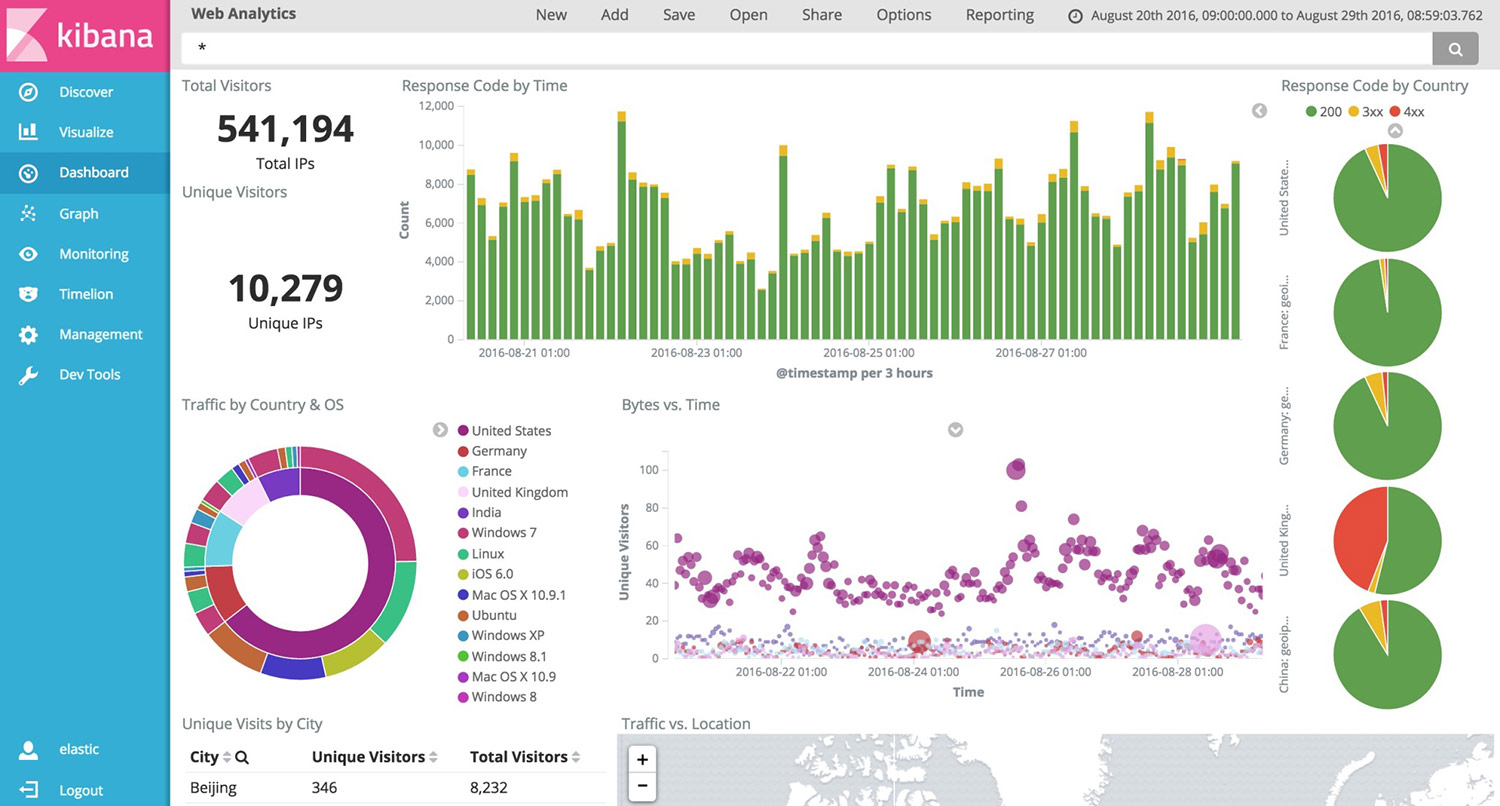
\includegraphics[scale=0.2]{kibana.jpg}
\caption{Exemple de tableau de bord Kibana}
\label{kibana}
\end{figure}

\subsection{Docker}

\begin{figure}[!h]
\centering
\def\svgwidth{0.5\columnwidth}
\input{images/docker.pdf_tex}
\caption{Le système de virtualisation Docker}
\label{docker}
\end{figure}

Docker est un système de virtualisation qui fonctionne par conteneurs. Son principal avantage est d'isoler les applications lancées dans ses conteneurs. Son utilisation dans le projet se justifie pour augmenter la tolérance aux pannes. En effet, il n'est pas souhaitable qu'une panne de Bro sur la passerelle Stargate oblige à redémarrer la machine. Cela engendrerait une coupure Internet indésirable pour les utilisateurs de la salle TIIR. Docker est donc une solution qui permet de ne pas impacter le reste du système en cas de dysfonctionnement d'un des conteneurs. Les applications lancées dans Docker sont Bro, Elasticsearch, Kibana et Logstash. Si l'un d'entre eux s'arrête il sera toujours possible d'utiliser les services des autres conteneurs. Si Logstash s'arrête, l'interface web Kibana fonctionnera toujours par exemple. La figure \ref{projet_final} montre le système et les différentes applications installées sur chacune des machines.

\begin{figure}[!h]
\centering
\def\svgwidth{\columnwidth}
\input{images/projet_final.pdf_tex}
\caption{Schéma du projet final}
\label{projet_final}
\end{figure}


%%% Local Variables:
%%% mode: latex
%%% TeX-master: "isae-report-template"
%%% End:
